\documentclass[11pt,]{article}
% \setcounter{tocdepth}{5}
% \setcounter{secnumdepth}{5}

\usepackage{hyperref}
\usepackage{cleveref}
\usepackage[T1]{fontenc}
\usepackage{amssymb,amsmath}
\usepackage{txfonts}
\usepackage{microtype}
\usepackage{amssymb,amsmath}
\usepackage{graphicx}
\usepackage{subfig} 
\usepackage{natbib}
\usepackage{paralist}
\usepackage{hyperref}
\usepackage{url}
\urlstyle{same}
\usepackage{color}
\usepackage{fancyvrb}
\usepackage[a4paper,body={170mm,250mm},top=25mm,left=25mm,head=14pt]{geometry}
\usepackage{fancyhdr}
\usepackage{xspace}
\xspaceaddexceptions{\%}
\renewcommand*\ttdefault{txtt} % 20% tighter than courier

%% uses fancyvrb
\newcommand{\VerbBar}{|}
\newcommand{\VERB}{\Verb[commandchars=\\\{\}]}
\DefineVerbatimEnvironment{Highlighting}{Verbatim}{commandchars=\\\{\}}
% Add ',fontsize=\small' for more characters per line

\newenvironment{Shaded}{}{}
\newcommand{\KeywordTok}[1]{\textcolor[rgb]{0.00,0.44,0.13}{\textbf{{#1}}}}
\newcommand{\DataTypeTok}[1]{\textcolor[rgb]{0.56,0.13,0.00}{{#1}}}
\newcommand{\DecValTok}[1]{\textcolor[rgb]{0.25,0.63,0.44}{{#1}}}
\newcommand{\BaseNTok}[1]{\textcolor[rgb]{0.25,0.63,0.44}{{#1}}}
\newcommand{\FloatTok}[1]{\textcolor[rgb]{0.25,0.63,0.44}{{#1}}}
\newcommand{\CharTok}[1]{\textcolor[rgb]{0.25,0.44,0.63}{{#1}}}
\newcommand{\StringTok}[1]{\textcolor[rgb]{0.25,0.44,0.63}{{#1}}}
\newcommand{\CommentTok}[1]{\textcolor[rgb]{0.38,0.63,0.69}{\textit{{#1}}}}
\newcommand{\OtherTok}[1]{\textcolor[rgb]{0.00,0.44,0.13}{{#1}}}
\newcommand{\AlertTok}[1]{\textcolor[rgb]{1.00,0.00,0.00}{\textbf{{#1}}}}
\newcommand{\FunctionTok}[1]{\textcolor[rgb]{0.02,0.16,0.49}{{#1}}}
\newcommand{\RegionMarkerTok}[1]{{#1}}
\newcommand{\ErrorTok}[1]{\textcolor[rgb]{1.00,0.00,0.00}{\textbf{{#1}}}}
\newcommand{\NormalTok}[1]{{#1}}

\hypersetup{breaklinks=true,
            pdfauthor={},
            pdftitle={},
            colorlinks=true,
            citecolor=blue,
            urlcolor=blue,
            linkcolor=magenta,
            pdfborder={0 0 0}}

\setlength{\parindent}{0pt}
\setlength{\parskip}{6pt plus 2pt minus 1pt}
\setlength{\emergencystretch}{3em}  % prevent overfull lines

\newcommand{\todo}[2]{{\textcolor{red}{\bf [#1] #2 }}\addcontentsline{toc}{subsubsection}{\textcolor{red}{[#1] #2} }}
\newcommand{\notes}[1]{\textcolor{blue}{\it #1 }}

\DeclareMathOperator{\softmax}{softmax}
\DeclareMathOperator{\sigmoid}{sigmoid}
\DeclareMathOperator{\sgn}{sgn}
\DeclareMathOperator{\relu}{relu}
\DeclareMathOperator{\lrelu}{lrelu}
\DeclareMathOperator{\elu}{elu}
\DeclareMathOperator{\selu}{selu}
\DeclareMathOperator{\maxout}{maxout}


%% uses fancyhdr
\pagestyle{fancy}

\author{}
\date{}



%% uses fancyhdr
\usepackage{titlesec}
\lhead{\sffamily MLP 2019/20:  Coursework 2}
\rhead{\sffamily Due: 22 November 2019}
\cfoot{\sffamily \thepage}
\crefformat{footnote}{#2\footnotemark[#1]#3}

\def\pagelimit{6\xspace}
\def\markweight{40\xspace}

\begin{document}

\begin{center}
\textsf{\textbf{\Large Machine Learning Practical 2019/20: Coursework 2}}

\bigskip
\textbf{Released: Monday 4 November 2019}

\textbf{Submission due: 16:00 Friday 22 November 2019}
\end{center}
\section{Introduction}
\label{sec:introduction}

The aim of this coursework is to further explore the classification of images using convolutional neural networks on a different dataset, \href{https://www.cs.toronto.edu/~kriz/cifar.html}{CIFAR100} (pronounced as ``see far 100''). CIFAR100 consists of 60,000 $32 \times 32$ colour images in 100 classes, with 600 images per class. The first part of the coursework will concern the implementation of convolutional networks using the MLP framework. The second part involves debugging and fixing a ``broken'' neural network, and then subsequently enhancing the resulting (now healthy) network to improve its generalization performance.

In order to support your experiments, we have acquired Google Cloud Platform credits which allow the use of the  \href{https://cloud.google.com/compute/docs/}{Google Compute Engine} infrastructure.
You will need to run the second part of the coursework (which will be carried out in \href{https://pytorch.org}{PyTorch}). Each student enrolled on the MLP course will receive a \$50 Google Cloud credit coupon which is enough to carry out the experiments required for this coursework. You will receive an email which will give you the URL you will need to access in order to request your Google Cloud Platform coupon. 

As in the previous coursework, you will need to submit your python code and a report.  In addition you will need to submit the outputs of test code that validates your implementation for the first part. The detailed submission instructions are given in Section \ref{sec:submission} -- please follow these instructions carefully.

\section{Github branch \texttt{mlp2019-20/coursework\_2}}
\label{sec:code}

The provided code and setup information for this coursework is available on the course
\href{https://github.com/CSTR-Edinburgh/mlpractical/}{Github repository}
on a branch \verb+mlp2019-20/coursework_2+. To create a local working
copy of this branch in your local repository you need to do the
following.

\begin{enumerate}
% \def\labelenumi{\arabic{enumi}.}
% \itemsep3pt\parskip0pt\parsep0pt
\item
  Make sure all modified files on the branch you are currently have been
  committed
  (see \href{https://github.com/CSTR-Edinburgh/mlpractical/blob/mlp2019-20/master/notes/getting-started-in-a-lab.md}{notes/getting-started-in-a-lab.md} if you are unsure how to do this).
\item
  Fetch changes to the upstream \texttt{origin} repository by running\\
  \texttt{git fetch origin}
\item
  Checkout a new local branch from the fetched branch using\\
  \verb+git checkout -b coursework_2 origin/mlp2019-20/coursework_2+
\end{enumerate}

You will now have a new branch in your local repository with everything you need to carry out the coursework.

Before continuing, remember to run \texttt{bash install.sh} to install some additional dependencies required. This assumes that you have already installed your environment as explained in \textbf{Lab1}, under \texttt{notes/environment-set-up.md}.

This branch includes the following additions to your setup:

\begin{itemize}
    \item For part 1:
    \begin{itemize}
        \item Updates to the \texttt{mlp} python modules including (in the \verb+mlp.layers+ module) the skeleton code of a \texttt{ConvolutionalLayer}.
        \item Jupyter notebooks, \texttt{ConvolutionalLayer\_tests.ipynb} for testing your implementations of convolutional layers, and supporting test code.
    \end{itemize}
    \newpage
     \item For part 2:
    \begin{itemize}
        \item A Jupyter notebook, \texttt{Coursework\_2\_Pytorch\_Introduction.ipynb}, which introduces Pytorch, and provides further resources on tutorials, documentation and debugging,
        \item A directory \texttt{pytorch\_mlp\_framework/}, which includes tooling and ready to run scripts to enable straightforward experimentation on GPU.  Documentation on this is included in  \texttt{notes/pytorch-experiment-framework.md}
        \item A note on how to use the Google Cloud Platform (using your student credits),\\\texttt{notes/google\_cloud\_setup.md}.
    \end{itemize}
     \item For the report:
    \begin{itemize}
        \item  A directory called  \texttt{report} which contains the LaTeX template and style files for your report.  You should copy all these files into the directory which will contain your report.
    \end{itemize}
\end{itemize}


\section{Tasks}
\label{sec:tasks}
This coursework comes in two parts. The objectives of the first part are
\begin{itemize} 
    \item To implement convolutional networks in the MLP framework,
    \item To validate your implementation using tests.
\end{itemize}

The objectives of the second part are:
\begin{itemize}
    \item To diagnose a deep CNN that cannot be properly trained due to optimization issues, and subsequently propose and implement solutions to the problem. Since the aim of this is to improve the \texttt{training} behaviour of the network, the solutions should then be evaluated in terms of {convergence speed} and {per-epoch training accuracy/loss}.
    \item To improve the generalization performance of the fixed network using both standard and more advanced methods (e.g. regularization, data augmentation etc).
\end{itemize}

Carrying out larger convolutional network experiments using the MLP numpy framework is computationally inefficient because (1) it runs on CPU and not on GPU, and (2) a  default implementation of a convolutional layer is unlikely to be computationally efficient. For these reasons the second part of the coursework, which involves running convolutional network experiments will use GPU computing (on the Google Compute Engine) and the highly efficient PyTorch framework.

\textbf{\emph{Please note that part 2 of the coursework does not depend on part 1. \\
Thus you can do them in either order (or simultaneously).}}

\subsection{Part 1:  Implementing convolutional networks in the MLP framework}
\label{sec:mlp}
In the first part of the coursework, you should implement convolutional layers in the MLP framework, and carry out some basic experiments to validate your implementation.

\begin{enumerate}
  \item We provide a convolutional layer skeleton as a class named \texttt{ConvolutionalLayer}.  This class should implement the methods \texttt{fprop}, \texttt{bprop} and \texttt{grads\_wrt\_params}.  There are two recommended approaches that you might consider to do the implementation (you only need to do the implementation using one of these approaches), based on
  \begin{compactitem}
      \item  the methods \texttt{scipy.signal.convolve2d} (and/or \texttt{scipy.signal.correlate2d});
      \item or using a ``serialisation'' approach using the method \texttt{im2col}.
  \end{compactitem}
  Both of these approaches are discussed below.
 
  \item Verify the correctness of your implementation using the supplied unit tests in the jupyter notebook file \texttt{notebooks/ConvolutionalLayer\_tests.ipynb} to verify your convolutional layer implementations. \textbf{Note:} The tests are not exhaustive and should serve only as an indication of going into the right direction. Ideally you should write additional tests to validate your code in other scenarios. Take special care to check for edge cases.

\item Generate and submit your personalised output files for the unit tests: \texttt{test\_convolution\_results\_pack.npz}\\
These files are automatically generated by activating your conda mlp environment, changing to the \texttt{scripts} directory in \texttt{mlpractical},  and running the following commands: 
 \begin{verbatim}
python generate_conv_layer_test_file.py --student_id sXXXXXXX
\end{verbatim}
Replace the \texttt{sXXXXXXX} with your student ID. Once the commands have run, the .npz file will be generated in the scripts folder. You should make sure that file is included as part of your submission (see Section~\ref{sec:submission}).
  
\item Since the required compute time for your convolutional network implementations will be substantial, it is \textbf{not} necessary/recommended to use this implementation to train and test convolutional networks on the CIFAR100 data.
\end{enumerate}

For part 1 you should submit  your code (in \texttt{mlp.layers}) and your output test files. There should also be a section of your report describing your implementation (either using pseudo-code or detailed verbal explanation) and including analysis of its computational efficiency.

\subsubsection{Implementing convolutional layers}

\textit{Time budget\footnote{\label{footnote:time-budget} These are simply suggested guidelines, feel free to adjust them based on your own preferences}: This section should take about 30\% of the time you have allocated for your coursework.}\newline

When you implement a convolutional layer, both the \texttt{fprop} and \texttt{bprop} methods can be based on a convolution operation, as explained in the lectures. If we consider the  \texttt{fprop} then the method operates on two 4-dimension tensors:
\begin{compactitem}
    \item The input (previous layer) to the convolution, whose dimensions are \texttt{(minibatch-size, num-feature-maps, $x_{in}$, $y_{in}$)};
    \item The kernels (weight matrices) for the convolutions,  whose dimensions are \texttt{(num-feature-maps-in, num-feature-maps-out, $x_{kernel}$, $y_{kernel}$)}.
\end{compactitem}

The key to implementing a convolutional layer is how the convolutions are implemented. We recommend that you consider one of the following approaches:
\begin{enumerate}
    \item Explicitly compute convolutions using the  SciPy convolution function \texttt{scipy.signal.convolve2d} (or \texttt{scipy.signal.correlate2d}).  Note that these functions convolve a 2-dimension image with a 2-dimension kernel, so your code will need to use this in the context of 4-dimension tensors where we have multiple feature maps and a batch of training examples.\newpage
    \item ``Serialisation'' in which the the convolution operation is turned into a single matrix multiplication.  The advantage of this is that implementing the convolutional \texttt{fprop} or \texttt{bprop} as a single large matrix multiplication is much more computationally efficient than the many small matrix multiplications a naive implementation would have.  The disadvantage of this approach is that the resultant matrix has repeated elements, and be large (dependent on the number of feature map, batch size, and image size).  
    
    This serialisation  approach uses a function called \texttt{im2col} (and its reverse \texttt{col2im}).  The \texttt{im2col} function is standard in Matlab and various computer vision packages, but it is not part of NumPy or SciPy; you may use the external Python implementations \texttt{im2col\_indices} and \texttt{col2im\_indices} at:\\ \url{https://github.com/huyouare/CS231n/blob/master/assignment2/cs231n/im2col.py}
\end{enumerate}

\emph{(25 Marks)}

\subsection{Part 2: Debugging training problems of a deep CNN and improving its generalization performance}
\label{sec:pytorch}
The second part of the coursework involves debugging and tuning deep CNNs using PyTorch and the Google Compute Engine.

Identifying and resolving any optimization-related problems that might prevent your model from fitting the training set are critical skills when working with deep neural networks. Furthermore once fitting is achieved as expected, it might still have severe overfitting problems, which cause low generalization performance. Being able to work around these two key problems is key to building high performance deep neural networks.

\begin{figure}
\centering
\begin{minipage}{.5\textwidth}
  \centering
  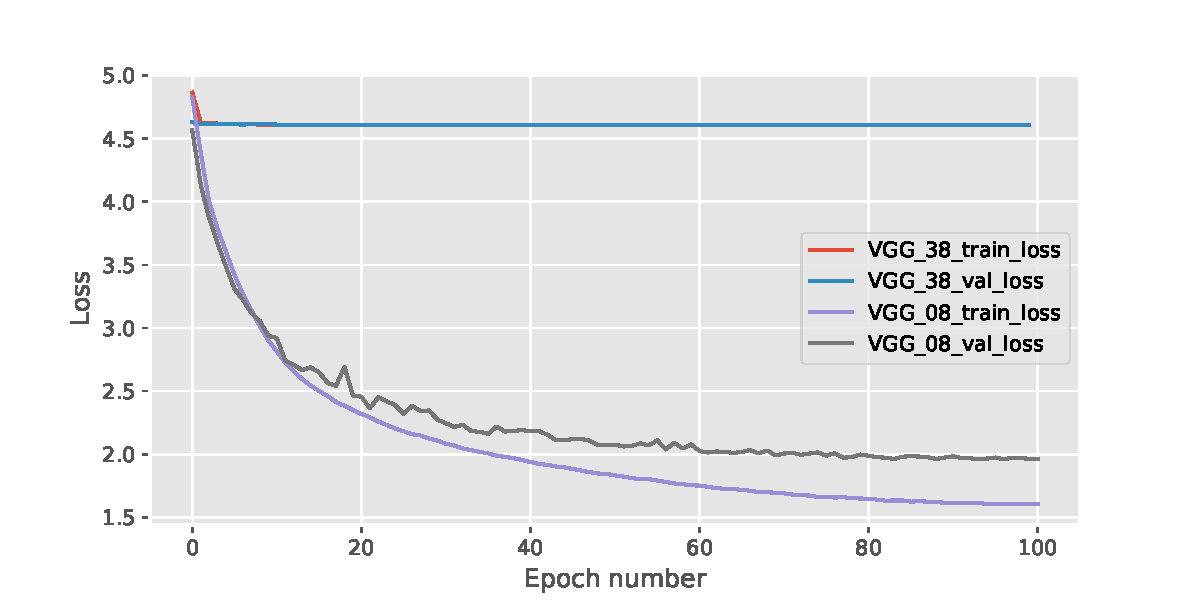
\includegraphics[width=1.1\linewidth]{loss_plot.pdf}
\end{minipage}%
\begin{minipage}{.5\textwidth}
  \centering
  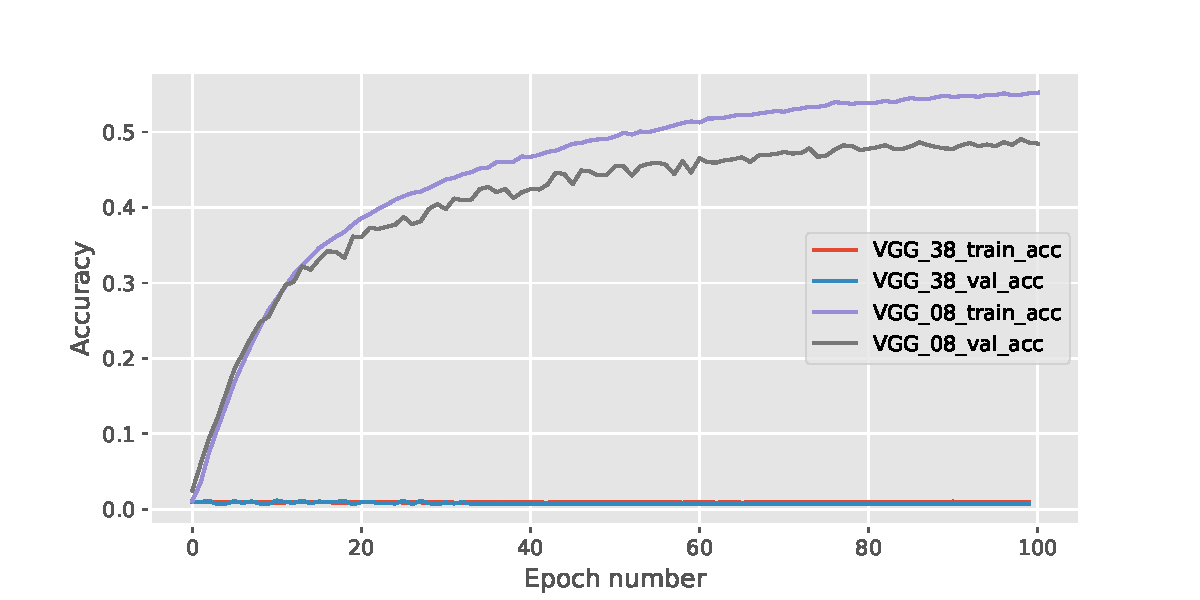
\includegraphics[width=1.1\linewidth]{accuracy_plot.pdf}
\end{minipage}
\caption{Training and validation plots of Healthy (VGG\_08) vs Broken (VGG\_38) in terms of error and accuracy.}
\label{brokenvshealthy}
\end{figure}

\subsubsection{Introducing our broken CNN}\label{broken-intro}

\textit{Time budget\cref{footnote:time-budget}: This section should take about 25\% of the time you have allocated for your coursework.}\newline

\textbf{Note: This section's objective is to test your knowledge, understanding and research skill. It's not meant to be an implementation-oriented section. The solutions require you to add at most 8-10 lines of code.}

Using the Pytorch-based research framework that can be found in the \texttt{pytorch\_mlp\_framework} folder, we have built, trained and evaluated 2 deep CNNs. One consisting of a total of 7 convolutional layers + one fully connected, and another consisting of 37 convolutional layers + one fully connected layer. Figure \ref{brokenvshealthy} illustrates the training/val loss performance of the two models. One can clearly see that the 37 layer CNN was unable to minimize its loss. Given that we know that extra layers means more abstraction power, parameters and capacity, one would expect the deeper model to be doing better at learning than the shallow one, however this is simply not the case. 

\subsubsection{Identifying and debugging the problem}\label{broken-high-level}

\begin{enumerate}
    \item Construct a hypothesis as to what is causing the issue in Figure \ref{brokenvshealthy}, as well as the collected metrics in folders \texttt{VGG\_08} and \texttt{VGG\_38}. Remember to support your position using arguments based on quantitative observations. 
    \item Propose 2 solutions to the problem. Implement your solutions using the provided research framework, and the guidelines in Section \ref{block-implementation-notes}. Design and run experiments that compare and contrast your proposed solutions, then discuss the results (Which one is better? Why? Is the problem partially or completely resolved?).
\end{enumerate}

\subsubsection{Implementation Guidelines}\label{block-implementation-notes}
There exist \emph{at least} several methods that can improve the training performance of the broken 37 layer CNN introduced in Section \ref{broken-intro}. The recommended solutions are described in 
\cite{ioffe2015batch, he2016deep}. You can also find alternative ones in \cite{huang2017densely, lee2015deeply} which can be more challenging to implement. We have written the MLP Pytorch framework in a way that allows you to implement said solutions with minimal effort. Each solution will require at approximately 2-8 lines of code. 

\textbf{Important Components to Note}

\begin{enumerate}
    \item The classes \texttt{ConvolutionalProcessingBlock} and \texttt{ConvolutionalDimensionalityReductionBlock} located within \texttt{pytorch\_mlp\_framework/model\_architectures.py}. The former class implements a basic cascade of 2 convolutional layers, each followed by a Leaky ReLU activation function, while the latter implements a basic cascade of 2 convolutional layers, with an average pooling layer in the middle, which effectively halves the height and width dimensions of the tensor volume passing through it. The former is used as the basic building block of the model (repeated \texttt{num\_blocks\_per\_stage times}), while the latter is used only as a dimensionality reduction layer, usually once after each \emph{network stage}. A network stage is considered a cascade of convolutional layers, followed by a dimensionality reduction function such as average pooling. 
    \item Lines 43-50 in \texttt{pytorch\_mlp\_framework/train\_evaluate\_image\_classification\_system.py} showcase how one can create an if-else structure that can read arguments from the command line in order to choose which processing and dim\_reduction blocks will be used.
    \item Lines 17-27 in the same file showcase how some simple data-augmentation strategies can be applied to the system (useful in improving the generalization of the model.)
     
\end{enumerate}

\textbf{Implementing a proposed solution}

\begin{enumerate}
    \item Copy the classes \texttt{ConvolutionalProcessingBlock} and \texttt{ConvolutionalDimensionalityReductionBlock} located within \texttt{pytorch\_mlp\_framework/model\_architectures.py}, and provide a name referring to your proposed solution. Then change the two blocks to implement your proposed solution.
    \item To create a new block ensure that you rewrite the \texttt{build\_module()} and \texttt{forward()} methods.
    \item Add a new clause in the if-else structure in lines 43-50 of  \texttt{pytorch\_mlp\_framework/train\_evaluate} \texttt{\_image\_classification\_system.py} to add a choice for a configuration using your new blocks.
    \item Write small unit-tests for your blocks to ensure that the layers can fprop some data without throwing errors related to Pytorch.
    \item Once tested, you can use the argument parser to easily run experiments with your new modules. Hint: Have a look at the \texttt{block\_type} argument under the \texttt{pytorch\_mlp\_framework}.
\end{enumerate}

\textbf{Note: Some potential solutions might not require modification of the above, but those are considered more advanced. If you choose that path, you will also bare the responsibility of figuring out the design of your code. That being said, most of known methods can be implemented using the above 3 steps.}

\subsubsection{Improving the generalization performance of the fixed model}   

\textit{Time budget\cref{footnote:time-budget}: This section should take about 5\% of the time you have allocated for your coursework.}\newline

\textbf{Note: If you were unable to debug the 37 layer deep CNN in the previous task, you can still get full marks on this section by improving the generalization performance of the 7 layer CNN. If you want to get more modelling capacity for your networks, simply increase the number of filters to 64. However, should you choose to do this, you'll need to run some baseline experiments on a 7 layer, 64 filter conv-net first, so you have something to compare against.}

Once a deep network is able to fit the training set at almost perfect performance, that's when we are ready to begin improving its generalization performance. This can be achieved with a variety of methods, some of which include regularization methods, data augmentation, special layer types, and various network topologies.
In this section your objective is to choose a few of such methods, implement them and compare their performance with each other. Finally, you should use what you've learned to build your final model, potentially combining some of the best methods you have experimented with, to get your final best test accuracy.

To break this down:

\begin{enumerate}
    \item Select a few methods targeted towards improving the generalization performance of the model, such as weight decay, L1/L2 regularization, dropout, data-augmentation etc.
    \item Implement selected methods. (Most of the above can be implemented using 1 line of code, or are already implemented into the framework, i.e. weight decay and some forms of data-augmentation).
    \item Design and run experiments to investigate the performance of the methods.
    \item Build a final model using the knowledge you have gained and evaluate its test performance.
    \item Write about what you did and why in your report.
\end{enumerate}

% \begin{enumerate}
%     \item We provide a Pytorch-based research framework that provides all the tooling and routines necessary to build, train, save and evaluate deep CNNs. This can be found in {missing}. Full information on how to use the framework can be found in {missing}.
%     \item 
% \end{enumerate}
% Explain why debugging optimization issues is important. Explain why knowing how to tune your network with standard or non-standard methods is also of extreme importance.

% Clearly state that they should design experiments or analyses that can probe into what's happening (remind that given figures contain enough information to at least suspect what the issue might be) and then clearly propose solutions and experiments that can clearly show that the network's issue was resolved.

% Introduce them to the framework, explain how one can run a simple experiment with the framework.

% Explain how they only need to copy 2 blocks, then edit the copied blocks and finally change 2 lines of code to exchange which modules are sent into the network. Tell them that they only need to add at most 7 lines of code in the blocks for their solutions, while most solutions require around 2-4 extra lines. 

% Ensure that they are aware of the goals of the coursework, which are for them to understand existing methods, design experiments and write a report. 
% Work on code framework, cross-reference stuff.
% Edit last years tutorial to add more information regarding the framework.

Note that the default hyperparameters (found in \texttt{arg\_extractor.py}) for provided in the framework (see\\ \texttt{pytorch\_experiment\_scripts/experiment\_builder.py}) are reasonable -- extensive hyperparameter searches are  not required in this coursework. 

Important things to note about experiments:
\begin{itemize}
    \item Your experiments should be designed so you are only varying one component at a time, so you can see the effect of that component-change.
    \item Designing experiments so that you are in a position to draw conclusions from your experiments is more important than the doing as many experiments as possible.
    \item When reporting the results of experiments, make sure that the comparison/contrast you are exploring is clear in the way you present the results.
\end{itemize}

Your report on this task should include the following:
\begin{itemize}
    \item \textbf{Introduction}.  Outline and explain the research questions you are investigating.  Provide citations if appropriate.
    \item \textbf{Methodology}.  Explain the methodology used -- in this case the approaches to modelling image context that have you explored.   Provide citations if appropriate.
    \item \textbf{Experiments}.  Describe carefully the experiments carried out, providing enough information to make them reproducible.  Present your results clearly and concisely.  Graphs and tables should be constructed to make clear the contrasts and comparisons you are interested in based on the research questions. For instance, some interesting evaluation criteria that can be used to compare different strategies are classification accuracy and speed of your network.
    \item \textbf{Discussion and conclusions.}  Discuss your results, with reference to the research questions, and if appropriate with reference to the literature.  What conclusions can you draw from your experiments and are they consistent with the literature?
\end{itemize}


\subsubsection*{Using Google Compute Engine}
\begin{enumerate}
    \item You will receive an email containing the URL you will need to access in order to request a Google Cloud Platform coupon, and information about how to do this.
    \item In the \texttt{coursework\_2} branch of the GitHub, \texttt{notes/google\_cloud\_setup.md} gives the instructions you should follow to set up a Google Compute Engine instance to carry out this coursework.
    \item The PyTorch experimental framework that is used for this coursework is described in\\\texttt{notes/pytorch-experiment-framework.md} and in\\\texttt{notebooks/Coursework\_2\_Pytorch\_experiment\_framework.ipynb}
\end{enumerate}

\emph{(75 Marks)}

\section{Report}
\label{sec:report}

\textit{Time budget\cref{footnote:time-budget}: The report should take about 40\% of the time you have allocated for your coursework.}\newline


Your coursework will be primarily assessed based on your submitted report.

The directory \verb+coursework_2/report+ contains a template for your report (\verb+mlp-cw2-template.tex+);  the generated pdf file (\verb+mlp-cw2-template.pdf+) is also provided, and you should read this file carefully as it contains some useful information about the required structure and content. The template is written in LaTeX, and we strongly recommend that you write your own report using LaTeX, using the supplied document style \verb+mlp2019+ (as in the template).

You should copy the files in the \verb+report+ directory to the directory containing the LaTeX file of your report, as \verb+pdflatex+ will need to access these files when building the pdf document from the LaTeX source file. The  \href{http://www.inf.ed.ac.uk/teaching/courses/mlp/2019-20/cw/mlp_cw1_2019_20.pdf}{coursework 1 spec} outlines how to create a pdf file from a LaTeX source file.

Your report should be in a 2-column format, based on the document format used for the ICML conference. The report should be a \textbf{maximum of \pagelimit pages long}, not including references.  We will not read or assess any parts of the report beyond this limit.

As discussed in the \href{http://www.inf.ed.ac.uk/teaching/courses/mlp/2019-20/cw/mlp_cw1_2019_20.pdf}{coursework 1 spec},  all figures should ideally be included in your report file as vector graphics files, rather than raster files as this will make sure all detail in the plot is visible.

% Matplotlib supports saving high quality figures in a wide range of
% common image formats using the
% \href{http://matplotlib.org/api/pyplot_api.html\#matplotlib.pyplot.savefig}{\texttt{savefig}}
% function. \textbf{You should use \texttt{savefig} rather than copying
% the screen-resolution raster images outputted in the notebook.} An
% example of using \texttt{savefig} to save a figure as a PDF file (which
% can be included as graphics in
% \href{https://en.wikibooks.org/wiki/LaTeX/Importing_Graphics}{LaTeX}
% compiled with \texttt{pdflatex} 
% %and in Apple Pages and \href{https://support.office.com/en-us/article/Add-a-PDF-to-your-Office-file-74819342-8f00-4ab4-bcbe-0f3df15ab0dc}{Microsoft Word} documents)
% is given below.

% \begin{Shaded}
% \begin{Highlighting}[]
% \CharTok{import} \NormalTok{matplotlib.pyplot }\CharTok{as} \NormalTok{plt}
% \CharTok{import} \NormalTok{numpy }\CharTok{as} \NormalTok{np}
% \CommentTok{# Generate some example data to plot}
% \NormalTok{x = np.linspace(}\DecValTok{0}\NormalTok{., }\DecValTok{1}\NormalTok{., }\DecValTok{100}\NormalTok{)}
% \NormalTok{y1 = np.sin(}\DecValTok{2}\NormalTok{. * np.pi * x)}
% \NormalTok{y2 = np.cos(}\DecValTok{2}\NormalTok{. * np.pi * x)}
% \NormalTok{fig_size = (}\DecValTok{6}\NormalTok{, }\DecValTok{3}\NormalTok{)  }\CommentTok{# Set figure size in inches (width, height)}
% \NormalTok{fig = plt.figure(figsize=fig_size)  }\CommentTok{# Create a new figure object}
% \NormalTok{ax = fig.add_subplot(}\DecValTok{1}\NormalTok{, }\DecValTok{1}\NormalTok{, }\DecValTok{1}\NormalTok{)  }\CommentTok{# Add a single axes to the figure}
% \CommentTok{# Plot lines giving each a label for the legend and setting line width to 2}
% \NormalTok{ax.plot(x, y1, linewidth=}\DecValTok{2}\NormalTok{, label=}\StringTok{'$y = \textbackslash{}sin(2\textbackslash{}pi x)$'}\NormalTok{)}
% \NormalTok{ax.plot(x, y2, linewidth=}\DecValTok{2}\NormalTok{, label=}\StringTok{'$y = \textbackslash{}cos(2\textbackslash{}pi x)$'}\NormalTok{)}
% \CommentTok{# Set the axes labels. Can use LaTeX in labels within $...$ delimiters.}
% \NormalTok{ax.set_xlabel(}\StringTok{'$x$'}\NormalTok{, fontsize=}\DecValTok{12}\NormalTok{)}
% \NormalTok{ax.set_ylabel(}\StringTok{'$y$'}\NormalTok{, fontsize=}\DecValTok{12}\NormalTok{)}
% \NormalTok{ax.grid(}\StringTok{'on'}\NormalTok{)  }\CommentTok{# Turn axes grid on}
% \NormalTok{ax.legend(loc=}\StringTok{'best'}\NormalTok{, fontsize=}\DecValTok{11}\NormalTok{)  }\CommentTok{# Add a legend}
% \NormalTok{fig.tight_layout()  }\CommentTok{# This minimises whitespace around the axes.}
% \NormalTok{fig.savefig(}\StringTok{'file-name.pdf'}\NormalTok{) }\CommentTok{# Save figure to current directory in PDF format}
% \end{Highlighting}
% \end{Shaded}


If you make use of any any books, articles, web pages or other resources
you should appropriately cite these in your report. You do not need to
cite material from the course lecture slides or lab notebooks.



% To create a pdf file \verb+mlp-cw2-template.pdf+ from a LaTeX source file (\verb+mlp-cw2-template.tex+), you can run the following in a terminal:
% \begin{verbatim}
% pdflatex mlp-cw2-template
% bibtex mlp-cw2-template
% pdflatex mlp-cw2-template
% pdflatex mlp-cw2-template
% \end{verbatim}
% (Yes, you have to run pdflatex multiple times, in order  for latex to construct the internal document references.)

% An alternative, simpler approach uses the \verb+latexmk+ program:
% \begin{verbatim}
% latexmk -pdf mlp-cw2-template
% \end{verbatim}

% Another alternative is to use an online LaTeX authoring environment such as \url{https://overleaf.com} -- note that all staff and students have free access to Overleaf Pro - see \url{https://www.ed.ac.uk/information-services/computing/desktop-personal/software/main-software-deals/other-software/overleaf}.

% It is worth learning how to use LaTeX effectively, as it is particularly powerful for mathematical and academic writing.  There are many tutorials on the web.


\section{Mechanics}
\label{sec:mechanics}

\textbf{Marks:} 
This assignment will be assessed out of 100 marks and forms \markweight\% of your final grade for the course.

\textbf{Academic conduct:} 
Assessed work is subject to University
regulations on academic
conduct:\\ {\small \url{http://web.inf.ed.ac.uk/infweb/admin/policies/academic-misconduct}}

\textbf{Submission:} 
You can submit more than once up until the submission deadline. All
submissions are timestamped automatically. Identically named files
will overwrite earlier submitted versions, so we will mark the latest
submission that comes in before the deadline.

If you submit anything before the deadline, you may not resubmit
after the deadline. (This policy allows us to begin marking submissions
immediately after the deadline, without having to worry that some may
need to be re-marked).

If you do not submit anything before the deadline, you may submit {\em
exactly once} after the deadline, and a late penalty will be applied
to this submission unless you have received an approved extension.
Please be aware that late submissions may receive lower priority for
marking, and marks may not be returned within the same timeframe as
for on-time submissions.

{\em Warning:} Unfortunately the \verb+submit+ command will technically
allow you to submit late even if you submitted before the deadline
(i.e.\ it does not enforce the above policy). Don't do this! We will
mark the version that we retrieve just after the deadline.

\textbf{Extension requests:} 
For additional information about late penalties and extension
requests, see the School web page below. \textbf{Do  not email any course
staff directly about extension requests as these are handled by the ITO; 
you must follow the instructions on the web page.}

{\small \url{http://web.inf.ed.ac.uk/infweb/student-services/ito/admin/coursework-projects/late-coursework-extension-requests}}

\textbf{Late submission penalty:}  
Following the University guidelines, 
late coursework submitted without an authorised extension will be
recorded as late and the following penalties will apply: 5
percentage points will be deducted for every calendar day or part
thereof it is late, up to a maximum of 7 calendar days. After this
time a mark of zero will be recorded.

\subsection{Backing up your work}
\label{sec:backing-up-your-work}

It is \textbf{strongly recommended} you use some method for backing up
your work. Those working in their AFS homespace on DICE will have their
work automatically backed up as part of the
\href{http://computing.help.inf.ed.ac.uk/backups-and-mirrors}{routine
backup} of all user homespaces. If you are working on a personal
computer you should have your own backup method in place (e.g.~saving
additional copies to an external drive, syncing to a cloud service or
pushing commits to your local Git repository to a private repository on
Github). \textbf{Loss of work through failure to back up
\href{http://web.inf.ed.ac.uk/infweb/student-services/ito/admin/coursework-projects/late-coursework-extension-requests}{does not constitute a good reason for
late submission}}.

You may \emph{additionally} wish to keep your coursework under version
control in your local Git repository on the \verb+coursework_2+ branch.

If you make regular commits of your work on the coursework this will
allow you to better keep track of the changes you have made and if
necessary revert to previous versions of files and/or restore
accidentally deleted work. This is not however required and you should
note that keeping your work under version control is a distinct issue
from backing up to guard against hard drive failure. If you are working
on a personal computer you should still keep an additional back up of
your work as described above.



\subsection{Submission}
\label{sec:submission}

Your coursework submission should be done electronically using the
\href{http://computing.help.inf.ed.ac.uk/submit}{\texttt{submit}}
command available on DICE machines.

Your submission should include

\begin{itemize}

\item
  your completed report as a PDF file, using the provided template
\item
  your local version of the \texttt{mlp} code including any changes
  you made to the modules (\texttt{.py} files)
 \item your personalised \texttt{test\_convolution\_results\_pack.npz} files. These can be automatically generated by activating your conda mlp environment and pointing your terminal to the directory \texttt{scripts} in the \texttt{mlpractical} repo and running the following commands: 
 \begin{verbatim}
python generate_conv_layer_test_file.py --student_id sXXXXXX
\end{verbatim}
Replace the sXXXXXXX with your student ID. Once the commands have been ran, the two .npz files will be generated under the scripts folder. You should make sure those files are included as part of your submission folder.

 \item your local version of the Pytorch experiment framework (\texttt{mlp/pytorch\_experiment\_scripts}), including any changes you've made to existing files and any newly created files.
 \item a copy of your Pytorch experiment directories, including \textbf{only} the \texttt{.csv} files for your training, validation and test statistics. Please do not include model weights.

\end{itemize}
Please do not submit anything else (e.g. log files).

You should copy all of the files to a single directory, \verb+coursework2+, e.g.

\begin{verbatim}
mkdir coursework2
cp reports/coursework2.pdf coursework2
cp scripts/test_convolution_results_pack.npz coursework2
\end{verbatim}
also copy to \texttt{coursework2} the directories containing your mlp and PyTorch code, as well as the directory containing the PyTorch \texttt{csv} files.
%cp sXXXXXXX_batchnorm_test_file.txt sXXXXXXX_conv_test_file.txt 


You should then submit this directory using

\begin{verbatim}
submit mlp cw2 coursework2
\end{verbatim}

\textbf{Please submit the directory, not a zip file, not a tar file.}

The \texttt{submit} command will prompt you with the details of the
submission including the name of the files / directories you are
submitting and the name of the course and exercise you are submitting
for and ask you to check if these details are correct. You should check
these carefully and reply \texttt{y} to submit if you are sure the files
are correct and \texttt{n} otherwise.

You can amend an existing submission by rerunning the \texttt{submit}
command any time up to the deadline. It is therefore a good idea
(particularly if this is your first time using the DICE submit
mechanism) to do an initial run of the \texttt{submit} command early on
and then rerun the command if you make any further updates to your
submission rather than leaving submission to the last minute.


\section{Marking Guidelines}
\label{sec:marking-scheme}
This document (Section \ref{sec:tasks} in particular) and the template report (\verb+mlp-cw1-template.pdf+) provide a description of what you are expected to do in this assignment, and how the report should be written and structured.

Assignments will be marked using the scale defined by the \textbf{University Common Marking Scheme}:
\begin{center}
\begin{tabular}{lll}
Numeric mark & Equivalent letter grade & Approximate meaning \\
$< 40$ & F & fail \\
40-49 & D & poor \\
50-59 & C & acceptable \\
60-69 & B & good \\
70-79 & A3 & very good/distinction \\
80-100 & A1, A2 & excellent/outstanding/high distinction
\end{tabular}
\end{center}

Please note the University specifications for marks above 70:

{\bf A1 90-100}
Often faultless. The work is well beyond what is expected for the level of study.

{\bf A2 80-89}
A truly professional piece of scholarship, often with an absence of errors. \\
As `A3' but shows (depending upon the item of assessment):
significant personal insight / creativity / originality
and / or
extra depth and academic maturity in the elements of assessment.

{\bf A3 70-79}\\
\emph{Knowledge}: Comprehensive range of up-to-date material handled in a professional way.\\
\emph{Understanding/handling of key concepts}: Shows a command of the subject and current theory.\\
\emph{Focus on the subject}: Clear and analytical; fully explores the subject.\\
\emph{Critical analysis and discussion}: Shows evidence of serious thought in critically evaluating and integrating the evidenced and ideas. Deals confidently with the complexities and subtleties of the arguments. Shows elements of personal insight / creativity / originality.\\
\emph{Structure}: Clear and coherent showing logical, ordered thought.\\
\emph{Presentation}: Clear and professional with few, relatively minor flaws. Accurate referencing. Figures and tables well constructed and accurate. Good standard of spelling and grammar.
\bibliographystyle{plainnat}
\bibliography{mlp-cw-references}
\end{document}
